\documentclass[10pt, a4paper, italian]{article}
\usepackage[T1]{fontenc}
\usepackage[utf8]{inputenc}
\usepackage{amsmath, amssymb, amsthm, thmtools, amsfonts, mathtools}
\usepackage{nicefrac}
\usepackage{calc}
\usepackage[pdftex, hyperindex, plainpages=false]{hyperref}
\usepackage[nameinlink]{cleveref} %load before classicthesis (clash)
%\usepackage[nochapters,pdfspacing]{classicthesis}
\usepackage{siunitx}
\usepackage[siunitx]{circuitikz}

\usepackage[a4paper]{geometry}
\usepackage{float}
\usepackage{mdframed}
\usepackage{titling}
\usepackage{booktabs}
\usepackage{graphicx}
\usepackage{caption, subcaption}
\usepackage{xcolor}
\usepackage[italian]{babel}
\usepackage{pgfplots}
\usepackage{listings}
%\usepackage{lmodern}
\usepackage{url}
\usepackage{enumitem}
\usepackage{tikz} %loads after classicthesis (xcolor incompat)

% lets graphicx know path where figures to be included are found
\graphicspath{{../figs/}}
\makeatletter
\def\input@path{{../figs/}}
%or: \def\input@path{{/path/to/folder/}{/path/to/other/folder/}}
\makeatother

% tikz pgf plots setup
\usepgfplotslibrary{external}
\pgfplotsset{compat=1.15}
%\tikzexternalize

% spaces and significant digits/figures for measurements
\sisetup{free-standing-units, space-before-unit, number-unit-product = \;,
scientific-notation = false, round-mode = figures, round-precision = 1,}

% turns all (hyperlinked) references black [default is blue]
\hypersetup{
	linktoc=all,
	colorlinks=true,
	linkcolor=black
}

% code listings config
%\lstset{
%language=Python,
%basicstyle=\ttfamily,
%columns=fullflexible,
%keepspaces=true,
%}

% mdframed (for boxed text) configuration
\mdfsetup{linewidth=0.6pt}

% Default fixed font does not support bold face
\DeclareFixedFont{\ttb}{T1}{txtt}{bx}{n}{12} % for bold
\DeclareFixedFont{\ttm}{T1}{txtt}{m}{n}{12}  % for normal

% Custom colors
\usepackage{color}
\definecolor{deepblue}{rgb}{0,0,0.5}
\definecolor{deepred}{rgb}{0.6,0,0}
\definecolor{deepgreen}{rgb}{0,0.5,0}

% Commands 
\newcommand{\executeiffilenewer}[3]{%
	\ifnum\pdfstrcmp{\pdffilemoddate{#1}}%
		{\pdffilemoddate{#2}}>0%
	{\immediate\write18{#3}}\fi%
}
% input .svg --> .pdf_tex graphs
%\newcommand{\includesvg}[1]{%
%	\executeiffilenewer{#1.svg}{#1.pdf}%
%	{inkscape -z -D --file=#1.svg %
%	--export-pdf=#1.pdf --export-latex}%
%	\input{#1.pdf_tex}%
%}
% Thanks UniPi's Department of Physics E. Fermi
\newcommand{\thanksdf}{(\thanks{Dipartimento di Fisica E.~Fermi,%
Universit\`a di Pisa - Pisa, Italy.}\;)}

% hyperlink to email address
\newcommand{\mail}[1]{\href{mailto:#1}{\textsf{#1}}}

% \vec for bold vectors, instead of overarrows (now "\arrvec")
\let\arrvec=\vec
\renewcommand{\vec}[1]{\boldsymbol #1}
% replaces straight phi with slanted phi
\renewcommand{\phi}{\varphi}
% replaces straight eps with curved epsilon
\newcommand{\eps}{\varepsilon}
% abbreviation for (sub_/super^)scripts of \lim, \sum,... in inline math
\newcommand{\ds}{\displaystyle}

% blackboard/number set letters
\newcommand{\CC}{\mathbb C}
\newcommand{\HH}{\mathbb H}
\newcommand{\KK}{\mathbb K}
\newcommand{\NN}{\mathbb N}
\newcommand{\PP}{\mathbb P}
\newcommand{\QQ}{\mathbb Q}
\newcommand{\RR}{\mathbb R}
\newcommand{\ZZ}{\mathbb Z}

\newcommand{\Abs}[1]{{\left\Vert #1\right\Vert}}
\newcommand{\enclose}[1]{{\left( #1 \right)}}
\newcommand{\Enclose}[1]{{\left[ #1 \right]}}
\newcommand{\floor}[1]{\left\lfloor #1 \right\rfloor}
\newcommand{\ceil}[1]{\left\lceil #1 \right\rceil}
\newcommand{\To}{\rightrightarrows}

% Math operators
\DeclareMathOperator{\divergence}{div}
\renewcommand{\div}{\divergence}
\DeclareMathOperator{\Imaginarypart}{Im}
\renewcommand{\Im}{\Imaginarypart}
\DeclareMathOperator{\Realpart}{Re}
\renewcommand{\Re}{\Realpart}
%\DeclareMathOperator{\arg}{arg}
\DeclareMathOperator{\tg}{tg}
\DeclareMathOperator{\arctg}{arctg}
\DeclareMathOperator{\settsinh}{settsinh}
\DeclareMathOperator{\settcosh}{settcosh}
\DeclareMathOperator{\tr}{tr}
\DeclareMathOperator{\im}{im}
\DeclareMathOperator{\sgn}{sgn}
\DeclareMathOperator{\diag}{diag}

\DeclarePairedDelimiter{\norm}{\lVert}{\rVert}
\DeclarePairedDelimiter{\scalar}{\langle}{\rangle}

% Logarithm with arbitrary base.
% -> log_10
\newcommand{\llog}[1][10]{\log_{#1}}

% Absolute value.
% -> |x|
\newcommand{\abs}[1]{\left| #1 \right|}

% Powers.
% -> x^a
\newcommand{\power}[2][2]{\left( #2 \right)^{#1}}

% Square.
% -> x^2
\newcommand{\sq}[1]{\power[2]{#1}}

% Expansion of the binomial coefficient.
% -> n1!/(n2!(n1 - n2)!)
\newcommand{\binomexpr}[2]{\frac{#1!}{#2!(#1 - #2)!}}

% Expression evaluation at a given point with square brackets.
% -> [x]_{a}
\newcommand{\at}[2]{\left[ #1\right]_{\makebox[-1pt][l]{${\scriptstyle#2}$}}}

% Expression evaluation in an interval.
% -> [x] _{a}^{b}
\newcommand{\eval}[3]{\left.#1%
  \right|_{\makebox[-1pt][l]{${\scriptstyle#2}$}}^{\makebox[-1pt][l]{${\scriptstyle#3}$}}}

% Upright d in math mode (for differentials).
% -> d
\newcommand{\ud}{\mathrm{d}}

% Differential.
% -> dx
\newcommand{\diff}[1][x]{\,\ud{#1}}

% Base command for defining derivatives.
% -> df/dx or d^kf/dx^k
\newcommand{\basederivative}[4][]{%
  \displaystyle%
  \ifx\\#1\\\frac{#4#2}{#4#3}%
  \else%
  \frac{#4^#1#2}{#4#3^#1}%
  \fi%
}

% Total derivative.
% -> df/dx(x) or d^kf/dx^k(x)
\newcommand{\td}[4][]{%
  \basederivative[#1]{#2}{#3}{\ud}%
  \ifx\\#4\\%
  \else%
  \mkern-4mu\left(#4\right)%
  \fi%
}

% Partial derivative.
% -> df/dx(x) or d^kf/dx^k(x)
\newcommand{\pd}[4][]{%
  \basederivative[#1]{#2}{#3}{\partial}%
  \ifx\\#4\\%
  \else%
  \mkern-4mu\left(#4\right)%
  \fi%
}

\newcommand{\intinf}{\int_{-\infty}^{\infty}\!\!\!}

\newcommand{\cinterval}[2]{\left[\, #1,~#2 \,\right]}

\newcommand{\linterval}[2]{\left[\, #1,~#2 \,\right)}

\newcommand{\rinterval}[2]{\left(\, #1,~#2 \,\right]}

\newcommand{\ointerval}[2]{\left(\, #1,~#2 \,\right)}

\newcommand{\prob}[1]{\displaystyle P\left(#1\right)}

\newcommand{\pvalue}{\emph{$p$-value}}

\newcommand{\cond}{\,|\,}

\newcommand{\expect}[1]{\displaystyle E\left[#1\right]}

\newcommand{\mom}[2][]{\displaystyle {\cal M}_{#2}\ifx\\#1\\\else(#1)\fi}

\newcommand{\momalg}[1]{\displaystyle \lambda_{#1}}

\newcommand{\momcen}[1]{\displaystyle \mu_{#1}}

\newcommand{\skewness}{\displaystyle \gamma_1}

\newcommand{\kurtosis}{\displaystyle \gamma_2}

\newcommand{\charf}[1][x]{\phi_{#1}}

\newcommand{\momgenf}[1][x]{M_{#1}}

\newcommand{\fwhm}{{\scriptstyle \textsc{FWHM}}}

\newcommand{\hwhm}{{\scriptstyle \textsc{HWHM}}}

\newcommand{\median}{\mu_{\nicefrac{1}{2}}}

\newcommand{\var}[1]{\ensuremath{\text{Var}\left(#1\right)}}

\newcommand{\cov}[2]{\ensuremath{\text{Cov}\left(#1, #2\right)}}

\newcommand{\corr}[2]{\ensuremath{\text{Corr}\left(#1, #2\right)}}

\newcommand{\like}{\mathcal L}

\newcommand{\likelihood}[2][]{\like\ifx\\#2\\\else(#2\ifx\\#1\\\else;#1\fi)\fi}

\newcommand{\chisq}{\ensuremath{\chi^2}}

\newcommand{\chisquare}[2][]{\chisq\ifx\\#2\\\else(#2\ifx\\#1\\\else;#1\fi)\fi}

\newcommand{\loglikelihood}[2][]{\log\likelihood[#1]{#2}}

\newcommand{\pdf}[3][]{#2(#3\ifx\\#1\\\else;#1\fi)}

\newcommand{\binomialpdf}[2][]{\pdf[#1]{\mathcal B}{#2}}

\newcommand{\multinomialpdf}[2][]{\pdf[#1]{\mathcal M}{#2}}

\newcommand{\poissonpdf}[2][]{\pdf[#1]{\mathcal P}{#2}}

\newcommand{\uniformpdf}[2][]{\pdf[#1]{u}{#2}}

\newcommand{\exponentialpdf}[2][]{\pdf[#1]{\varepsilon}{#2}}

\newcommand{\gausspdf}[2][]{\pdf[#1]{N}{#2}}

\newcommand{\chisquarepdf}[2][]{\pdf[#1]{\wp}{#2}}

\newcommand{\cauchypdf}[2][]{\pdf[#1]{c}{#2}}

\newcommand{\erf}[1]{\ensuremath{\text{erf}\left(#1\right)}}

\newcommand{\dccases}[4][]{#2 \ifx\\#2\\\else=\fi %
  \begin{cases}
    \displaystyle #3 & \text{per variabili discrete}\\
    \displaystyle #4 & \text{per variabili continue}#1
  \end{cases}
}
% sub/super-scriptable for all symbol as math operator 
\newcommand\Scaleforall[1]{\vcenter{\hbox{\scalefont{#1}$\forall$}}}

\DeclareMathOperator*\forevery{%
  \vphantom\sum
  \mathchoice{\Scaleforall{2}}{\Scaleforall{1.4}}{\Scaleforall{1}}{\Scaleforall{0.75}}}
\usepackage{multicol}
\geometry{left=2cm, right=2cm, top=2cm, bottom=2cm}
\usepackage{colortbl}
\usepackage{diagbox}
\usepackage[T1]{fontenc}
\usepackage[utf8]{inputenc}
\usepackage{graphicx}
\usepackage{xcolor}
\usepackage{tkz-graph}
\usepackage{arydshln}
\usetikzlibrary{automata, positioning, arrows}
\newenvironment{FSM}{
\begin{tikzpicture}
\tikzset{
->, % makes the edges directed
>=stealth', % makes the arrow heads bold
node distance=2cm, % specifies the minimum distance between two nodes. Change if necessary.
every state/.style={minimum size = 1cm, thick, fill=gray!10}, % sets the properties for each 'state' node
}
}{
\end{tikzpicture}
}


\lstset{%
  language = Octave,
  backgroundcolor=\color{white},   
  basicstyle=\footnotesize\ttfamily,       
  breakatwhitespace=false,         
  breaklines=true,                 
  captionpos=b,                   
  commentstyle=\color{gray},    
  deletekeywords={...},           
  escapeinside={\%*}{*)},          
  extendedchars=true,              
  frame=single,                    
  keepspaces=true,                 
  keywordstyle=\color{orange},       
  morekeywords={*,...},            
  numbers=left,                    
  numbersep=5pt,                   
  numberstyle=\footnotesize\color{gray}, 
  rulecolor=\color{black},         
  rulesepcolor=\color{blue},
  showspaces=false,                
  showstringspaces=false,          
  showtabs=false,                  
  stepnumber=2,                    
  stringstyle=\color{orange},    
  tabsize=2,                       
  title=\lstname,
  emphstyle=\bfseries\color{blue}%  style for emph={} 
} 

%% language specific settings:
\lstdefinestyle{Arduino}{%
    language = Octave,
    keywords={void, int boolean},%                 define keywords
    morecomment=[l]{//},%             treat // as comments
    morecomment=[s]{/*}{*/},%         define /* ... */ comments
    emph={HIGH, OUTPUT, LOW}%        keywords to emphasize
}

% indexes subsections with letters, sections with numbers (1.a, 1.b, ...)
\renewcommand{\thesubsection}{\thesection.\alph{subsection}}

% lets graphicx know path where figures to be included are found
\graphicspath{{../figs/}}

\newcommand{\dontcare}{X}
\author{Gruppo 1.AC \\ Matteo Rossi, Bernardo Tomelleri}
\title{EsD4 ADC-DAC: Convertitore sigma-delta}
\begin{document}
\date{\today}
\maketitle

\section*{Misura componenti dei circuiti}
Riportiamo per completezza il valore della tensione continua di
alimentazione per i circuiti integrati misurata con il multimetro
\[
V_{CC} = 4.99 \pm 0.03 \; \si{\V}
\]

e il valore di capacità del condensatore di disaccoppiamento che collega le
linee di alimentazione a massa (sempre misurato con il multimetro)
\[
C_d = 97 \pm 4 \; \si{n\F}
\]

\setcounter{section}{0}

%=======================
\section{Analisi e costruzione del circuito}\label{sec: IC}
Si vuole costruire una macchina a stati finiti in grado di emulare il
funzionamento delle luci di un semaforo stradale, nelle modalità
\begin{description}
\item[ABILITATO] si ripetono in ciclo gli stati: LED verde acceso $\to$
LED giallo e verde accesi $\to$ LED rosso acceso.
\item[DISABILITATO] si alternano gli stati LED giallo acceso e spento
(giallo lampeggiante).
\end{description}
in cui tutti gli stati hanno durata pari ad un impulso del clock inviato
all'ingresso dei circuiti integrati a disposizione.

%=======================
\section{Descrizione delle misure e acquisizione dati}
Si vuole ricostruire il circuito precedente per il controllo di un semaforo
tramite un microcontrollore (nel nostro caso utilizzeremo Eleego UNO R3).
\begin{figure}[htbp]
    \centering
%    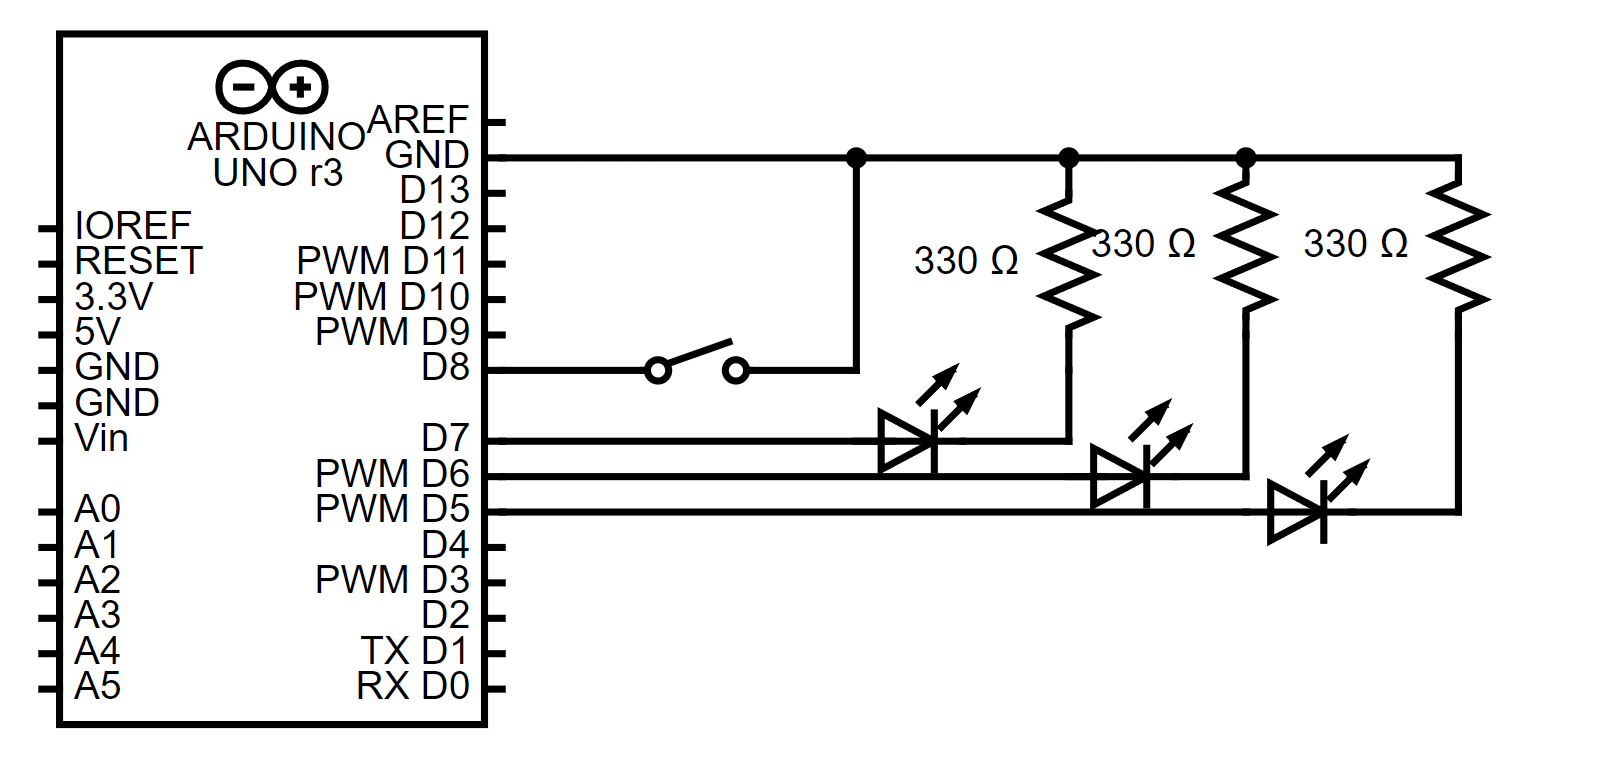
\includegraphics[width=\textwidth]{schem_ard}
    \caption{Schematica utilizzata per la gestione del semaforo con software
    tramite Eleego.
    \label{schem: arduino}}
\end{figure}
Dopo aver assemblato il circuito descritto in \cref{schem: arduino}, si
procede con l'implementazione software del semaforo.

\subsection{Definizione del segnale in ingresso}
Ci basiamo sullo schema per il semaforo FSM di Mealy presente in
\cref{diag: semf} per controllare il funzionamento del semaforo tramite
segnale di controllo ENABLE, riportiamo il listato del programma nel listing

\subsection{Campionamento e acquisizione del segnale}
Si introduce un quarto stato nel caso in cui il semaforo sia abilitato,
successivo al rosso; per fare ciò è necessaria una semplice modifica
all'interno dello switch nel caso in cui il semaforo risulti abilitato.
Riportiamo le modifiche apportate al codice precedente nel listing
\ref{list: sviz}.
\begin{lstlisting}[label={list: sviz}, style=Arduino, caption=Svizzero.ino]
void loop() {
  //viene controllato se il semaforo \'e abilitato
  if(CheckEnable()){ 
    
    // nel caso in cui il semaforo sia abilitato
    switch(CurrentState){  
    case 1://se lo stato precedente risulta essere solo rosso
      CurrentState=2;
      digitalWrite(6,HIGH); //imposta lo stato corrente a rosso e giallo
      delay(tickREDYELLOW); //viene fatto passare il tempo specificato all'inizio del file
      break;
    case 2: //se lo stato precedente risulta essere rosso e giallo
      CurrentState=3; //lo stato corrente viene spostato a verde
      digitalWrite(5,LOW);
      digitalWrite(6,LOW);
      digitalWrite(7,HIGH);  
      delay(tickGREEN); 
      break; 
    .
    .
    .
\end{lstlisting}

\subsection{Acquisizione con Protocol}

%=======================
\section{Analisi dei dati}
Si vuole realizzare una FSM che riceve uno stream di bit su una linea di
ingresso e che accende un LED tutte le volte che su questo si presenta un
fronte di discesa secondo il modello di Moore e un'altra secondo quello di
Mealy.

\subsection{Ricostruzione dei segnali in ingresso}
Seguendo lo stesso procedimento usato nella \cref{sec: IC} per realizzare il
semaforo disegniamo i diagrammi degli stati delle macchine, ne codifichiamo in
bit gli stati, ricaviamo le tabella di verità per le transizioni tra questi e
i valori in uscita, così da ottenere le equazioni logiche che le governano da
tradurre nella realizzazione pratica delle connessioni tra memoria e circuiti
di logica combinatoria.

\subsection{Fit sinusoidale}
Si è scelto di costruire la FSM di Moore per riconoscere fronti di discesa
con 3 stati, dunque 2 bit di memoria $Q_1 Q_0$ secondo il diagramma degli
stati in \cref{diag: edgeMoore}. Per cui se il segnale di rumore in ingresso
rimane a livello logico basso o alto la macchina resta in stato LOW $(00)$ o
HIGH $(01)$ in cui l'uscita è OUT~$= 0$;
se invece il segnale IN scende a 0 durante lo stato HIGH la macchina entra
nell'unico stato (EDGE $\coloneqq 10$) in cui l'uscita è OUT~$= 1$ prima di
tornare ad uno degli stati precedenti a seconda del valore logico
dell'ingresso al successivo fronte di salita del clock.
\begin{figure}[htbp]
\centering
\begin{FSM}
\tikzset{node distance = 4cm, on grid, auto
}
\node (H) [state with output] {HIGH \nodepart{lower} $01$};
\node (C) [state with output, right of = H] {EDGE \nodepart{lower} $10$};
\node (L) [state with output, right of = C] {LOW \nodepart{lower} $00$};
 
\path [-stealth, thick]
	(H) edge [loop left]  node {IN=1}()
    (H) edge [bend left] node[above] {IN=0} (C)
    (C) edge [bend left] node[above] {IN=1} (H)
    (C) edge [bend left] node[above] {IN=0} (L)
    (L) edge [bend left] node {IN=1} (H)
    (L) edge [loop right]  node {IN=0}();
\end{FSM}
\caption{Edge-detector FSM di Moore
\label{diag: edgeMoore}}
\end{figure}

Dal diagramma ricaviamo la tabella di verità delle transizioni di stato con
la stessa convenzione usata prima tra lo stato corrente $Q_i$ e il successivo
$D_i$ come riportata in \cref{tab: bitMoore}.
\begin{table}[htbp]
\centering
\begin{tabular}{c:c|cc||cc|c}
\toprule
State & IN & $Q_1$ & $Q_0$ & $D_1$ & $D_0$ & OUT \\
\midrule
\midrule
LOW   & 0  & 0  & 0  & 0  & 0  & 0   \\
      & 1  & 0  & 0  & 0  & 1  & 0   \\
\midrule
EDGE  & 0  & 1  & 0  & 0  & 0  & 1   \\
      & 1  & 1  & 0  & 0  & 1  & 1   \\
\midrule
HIGH  & 0  & 0  & 1  & 1  & 0  & 0   \\
      & 1  & 0  & 1  & 0  & 1  & 0   \\
\bottomrule
\end{tabular}
\caption{Tabella di verità per le transizioni tra gli stati del detector di
Moore. \label{tab: bitMoore}}
\end{table}

Dunque per semplificare le espressioni logiche delle transizioni e delle
uscite si sono costruite le mappe di Karnaugh riportate in
\cref{tab: KarD0edge}, \cref{tab: KarD1edge} e \cref{tab: KarOUT}.
\begin{table}[htbp]
\centering
	\begin{tabular}{c|c|c|c|c}
        \backslashbox{IN}{$Q_1 Q_0$} & 00 & 01 & 11 & 10\\
        \hline
        0 & 0 & 0 & X & 0 \\
        \hline
        1 & 1 & 1 & X & 1 \\
    \end{tabular}
	\caption{Mappa di Karnaugh per $D_0 = \text{IN}$
	 \label{tab: KarD0edge}}

\bigskip
	 
    \begin{tabular}{c|c|c|c|c}
        \backslashbox{IN}{$Q_1 Q_0$} & 00 & 01 & 11 & 10\\
        \hline
        0 & 0 & \cellcolor[HTML]{FF9999} 1 & \cellcolor[HTML]{FF9999} X & 0 \\
        \hline
        1 & 0 & 0 & X & 0 \\
    \end{tabular}
	\caption{Mappa di Karnaugh per $D_1 = \overline{\text{IN}} \cdot Q_0$
	 \label{tab: KarD1edge}}

\bigskip

    \begin{tabular}{c|c|c|c|c}
        \backslashbox{IN}{$Q_1 Q_0$} & 00 & 01 & 11 & 10\\
        \hline
        0 & 0 & 0 & \cellcolor[HTML]{FF9999} X & \cellcolor[HTML]{FF9999} 1 \\
        \hline
        1 & 0 & 0 & \cellcolor[HTML]{FF9999} X & \cellcolor[HTML]{FF9999} 1 \\
    \end{tabular}
    \caption{Mappe di Karnaugh per $\text{OUT} = Q_1$
    \label{tab: KarOUT}}
\end{table}

Finalmente dalle equazioni per gli stati futuri e delle uscite della FSM
si è costruito il circuito riportato in \cref{schm: edgeMoore} a partire da
due positive-edge-triggered D Flip-Flop (IC 74LS74), 1 porta AND (74LS08) e
una porta NOT (74LS04).
\begin{figure}[htbp]
    \centering
    \begin{circuitikz}
    \tikzset{flipflop D/.style={flipflop,
    flipflop def={t1=$D_0$, t6=$Q_0$, c3=1, t4=\ctikztextnot{$Q_0$}}},
	}
        \def\andScale{0.7};

        % componenti
        %% flip flop
        \draw (0,0) node[flipflop D] (ffSinistra) {};
		\tikzset{flipflop D/.style={flipflop,
		flipflop def={t1=$D_1$, t6=$Q_1$, c3=1, t4=\ctikztextnot{$Q_1$}}},
		}
        \draw (5,0) node[flipflop D] (ffDestra) {};
        
        %% and gate
        \node (andDestra) at (3, |- ffDestra.pin 1) [and port, scale=\andScale] {};
        \node at (andDestra.bin 1) [ocirc, left] {};
        
        % input
        \node (IN) at ($ (ffSinistra.pin 1) + (-2,1) $) {IN};
        \node (CLK) at ($ (IN) + (0,-4) $) {CLK};
        \draw (9.5,-1.5) node[eground] (gnd){};

        % fili
        %% clock e in
        \draw (CLK) -| (ffDestra.pin 3);
        \draw (ffSinistra.pin 3) -- (ffSinistra.pin 3 |-, |- CLK);
        \draw (IN) -| (andDestra.in 1);
        \draw (ffSinistra.pin 1) -- (ffSinistra.pin 1 |-, |- IN);
        \draw (ffSinistra.pin 6) |- (andDestra.in 2);
        
        \draw (andDestra.out) -- (ffDestra.pin 1);
        \draw (ffDestra.pin 6) to
        [/tikz/circuitikz/bipoles/length=1cm,empty led, l=OUT]
        ++ (1.5,0) to[/tikz/circuitikz/bipoles/length=1cm, R,l=\SI{1}{\kilo\ohm}]
        ++ (1.5,0) -| (gnd);
    \end{circuitikz}
    \caption{schema del detector Moore.
    \label{schm: edgeMoore}}
\end{figure}

\subsection{Risposta in frequenza dell'ADC}
Per la realizzazione della FSM di Mealy per riconoscere fronti di discesa
invece sono sufficienti 2 stati, quindi 1 bit di memoria, come si vede anche
dal diagramma degli stati riportato in \cref{diag: edgeMealy}. Anche in questo
caso il segnale di rumore viene inviato all'ingresso $D$ del FF, ma ora viene
comparato continuamente con lo stato precedentemente registrato in
memoria $Q$. Dunque il valore in uscita dal circuito è sempre OUT~$= 0$
apparte quando la macchina registra la discesa del segnale IN a 0 durante lo
stato HIGH $(Q = 1)$, per cui OUT: $0 \to 1$ lungo il fronte di discesa del
segnale di clock.
\begin{figure}[htbp]
\centering
\begin{FSM}
\tikzset{node distance = 4cm, on grid, auto
}
\node (H) [state] {HIGH};
\node (L) [state, right of = H] {LOW};
 
\path [-stealth, thick]
	(H) edge [loop left]  node {IN$=1$ (OUT$=0$)}()
    (H) edge [bend left] node[above] {IN$=0$ (OUT$=1$)} (L)
    (L) edge [bend left] node {IN$=1$ (OUT$=0$)} (H)
    (L) edge [loop right]  node {IN$=0$ (OUT$=0$)}();
\end{FSM}
\caption{Edge detector FSM di Mealy
\label{diag: edgeMealy}}
\end{figure}

Come prima ricaviamo dal diagramma la tabella di verità delle transizioni di
stato riportata in \cref{tab: bitMealy} con le solite convenzioni; stavolta
non è necessario ricorrere alle mappe di Karnaugh per semplificare le
espressioni dello stato futuro $D =$ IN e dell'uscita OUT
$= \overline{\text{IN}} \cdot Q$
\begin{table}[htbp]
	\centering
	\begin{tabular}{cc|c}
	\toprule
	$D$ = IN & $Q$ & OUT \\
	\midrule
	\midrule
	$0$  & $0$	& $0$ \\
	$0$  & $1$	& $1$ \\
	$1$  & $0$	& $0$ \\
	$1$  & $1$  & $0$ \\
	\bottomrule
	\end{tabular}
	\caption{codifica binaria degli stati del detector di Mealy.
	$D$ = IN; OUT = $\overline{\text{IN}} \cdot Q$
	\label{tab: bitMealy}}
\end{table}

A partire da queste equazioni si è costruito il circuito riportato in
\cref{schm: edgeMealy} con un positive-edge-triggered D Flip-Flop (IC 74LS74),
1 porta AND (74LS08) e una porta NOT (74LS04).
\begin{figure}[htbp]
    \centering
    \begin{circuitikz}
	\def\andScale{0.7};
        % componenti
        %% flip flop
        \draw (0,0) node[flipflop D] (ffSinistra) {};
        
        %% and gate
        \node (andDestra) at ($ (ffSinistra.pin 6) + (1.5,0.2) $) [and port, scale=\andScale] {};
        \node at (andDestra.bin 1) [ocirc, left] {};
        
        % input
        \node (IN) at ($ (ffSinistra.pin 1) + (-2,1) $) {IN};
        \node (CLK) at ($ (ffSinistra.pin 3) + (-2,0) $) {CLK};
        \draw (6.5,-1) node[eground] (gnd){};

        % fili
        %% clock e in
        \draw (CLK) -| (ffSinistra.pin 3);
        \draw (IN) -| (andDestra.in 1);
        \draw (ffSinistra.pin 1) -- (ffSinistra.pin 1 |-, |- IN);
        \draw (ffSinistra.pin 6) |- (andDestra.in 2);
        
        \draw (andDestra.out) to
        [/tikz/circuitikz/bipoles/length=1cm,empty led, l=OUT]
        ++ (1.5,0) to[/tikz/circuitikz/bipoles/length=1cm, R,l=\SI{1}{\kilo\ohm}]
        ++ (1.5,0) -| (gnd);
    \end{circuitikz}
    \caption{schema del detector Mealy.
    \label{schm: edgeMealy}}
\end{figure}

\subsection{Stima del fattore di calibrazione del convertitore}
Con la funzione Patterns di Waveform si invia un segnale (in DIO 5) di clock
di frequenza $f\ped{clk} = \SI{1}{k\Hz}$ al pin (CLK) dei Flip-Flop e si
genera con il canale DIO 6 uno stream di dati random alla stessa frequenza
$f = f\ped{clk}$, già dalla schermata di Patterns è possibile notare come
le commutazioni di stato del segnale pseudocasuale avvengano in corrispondenza
dei fronti di discesa del segnale di clock.

Come prima si sono mantenuti i pin PRESET e CLEAR dei D-FF collegati a
$V_{CC}$ per evitare reset o clear spuri.

\subsection{Misura del signal/noise ratio (SNR)}
Si sono acquisiti i segnali in ingresso (CLK = DIO 5, IN = DIO 6) e in uscita
(OUT = DIO 7) dai circuiti edge-detector con la funzione Logic Analyzer
dell'AD2, di cui riportiamo i risultati per il circuito di Moore in
\cref{fig: edgeMoore} e per la FSM di Mealy in \cref{fig: edgeMealy}.
\begin{figure}[htbp]
    \centering
%    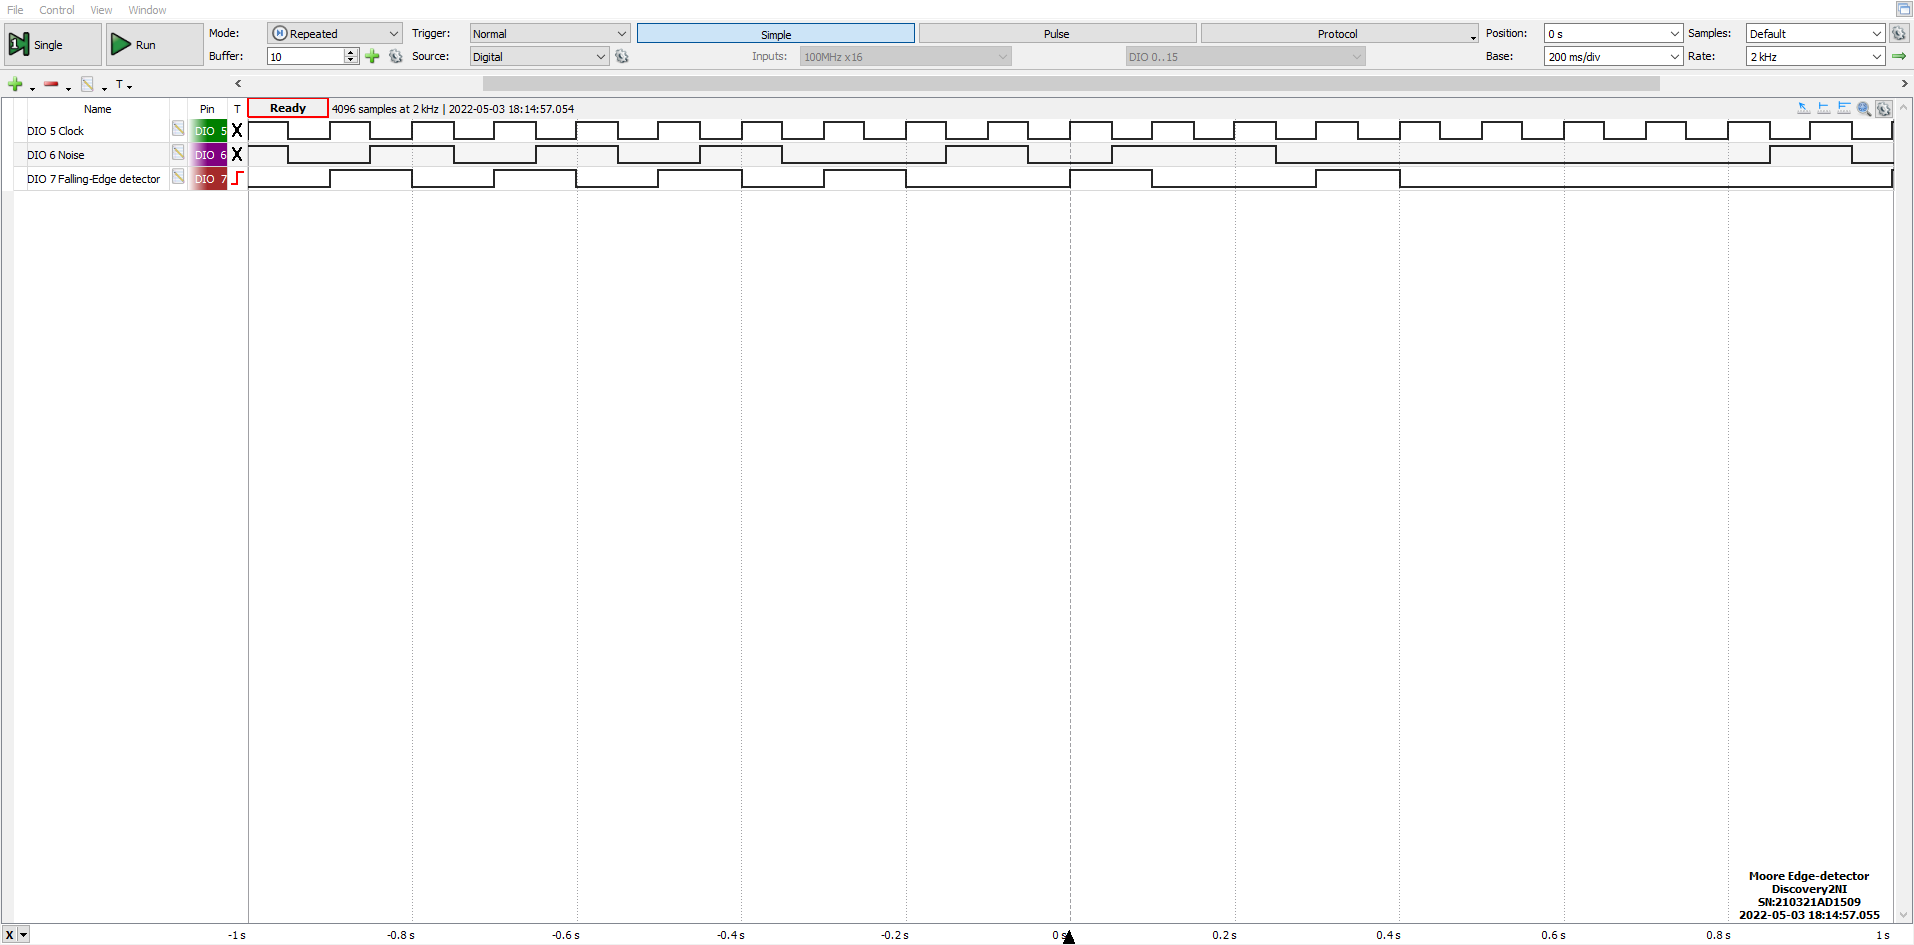
\includegraphics[width=\textwidth]{Moore_edge_detector}
    \caption{Acquisizione di un ciclo completo (frequenza 1 kHz) con Logic
    Analyzer dei segnali in ingresso e in uscita dall'edge detector di Moore.
    \label{fig: edgeMoore}}
\end{figure}

Notiamo nel primo caso come l'uscita assume valore alto in maniera sincrona
rispetto al fronte di salita del segnale di clock, mentre nell'implementazione
di Mealy l'uscita sale in maniera sincrona rispetto al fronte di discesa del
segnale di rumore IN.
\begin{figure}[htbp]
    \centering
%    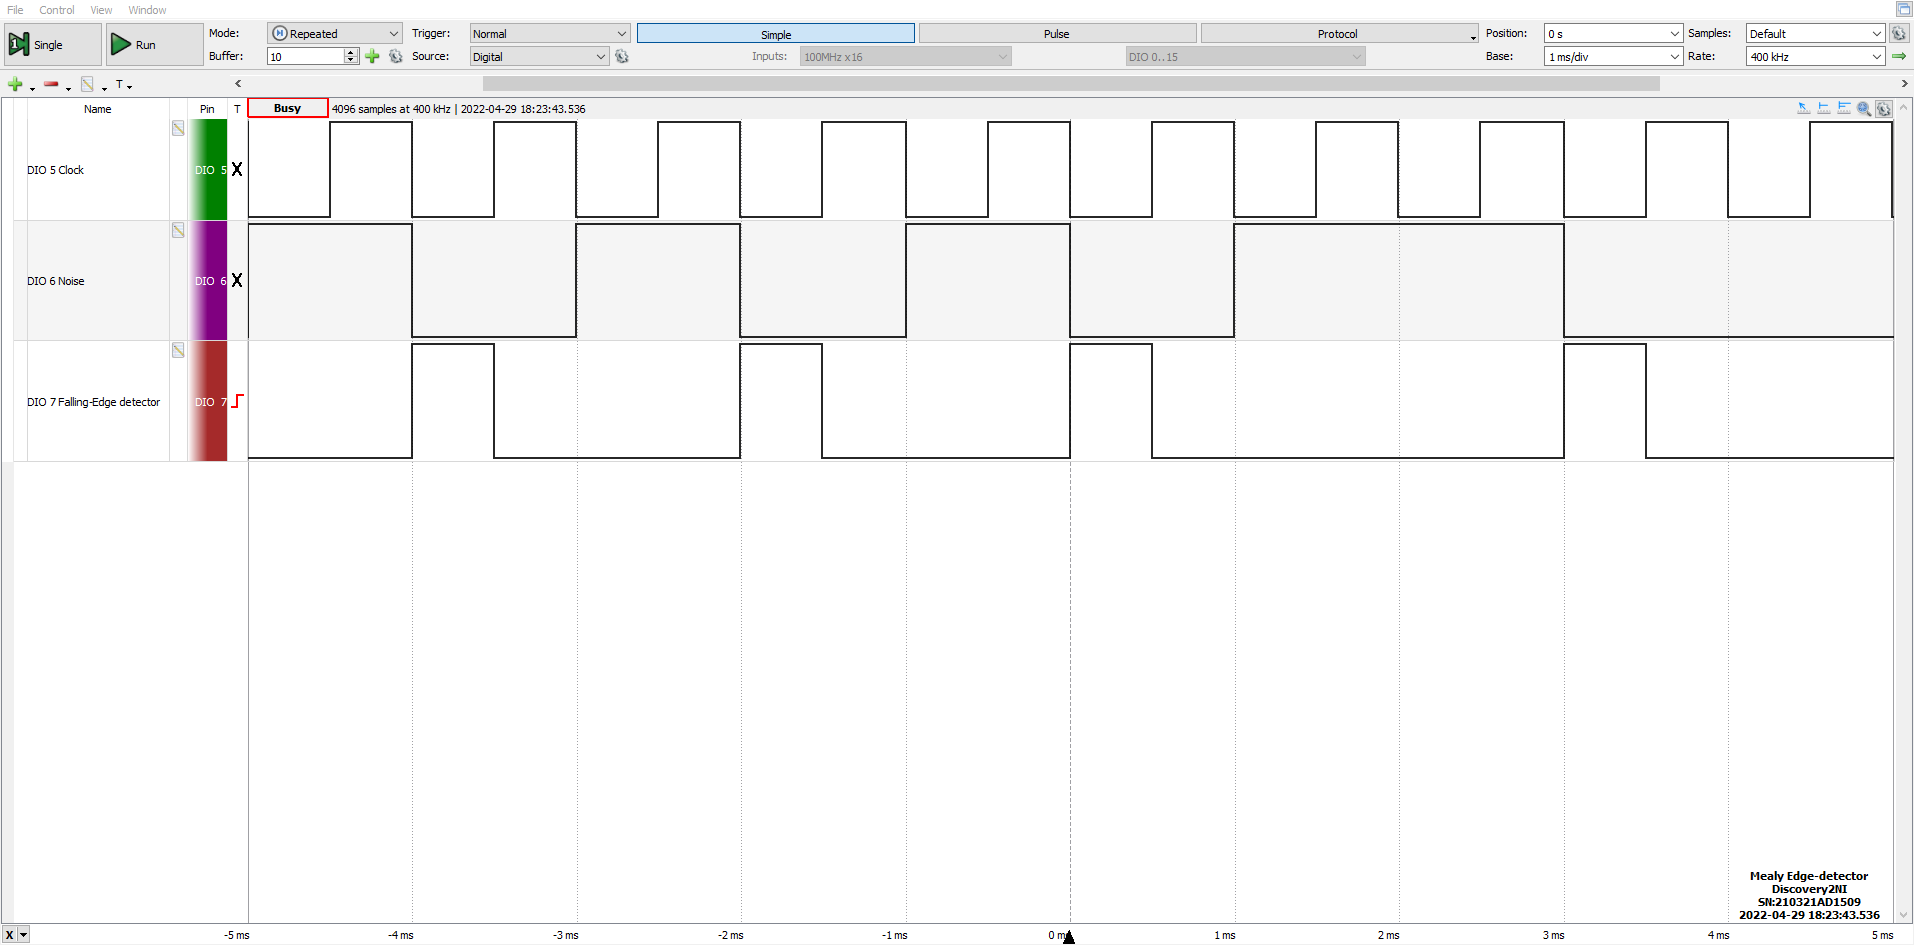
\includegraphics[width=\textwidth]{Mealy_edge_detector}
    \caption{Acquisizione di un ciclo completo (frequenza 1 kHz) con Logic
    Analyzer dei segnali in ingresso e in uscita dal detector di Mealy.
    \label{fig: edgeMealy}}
\end{figure}

Questo risulta compatibile con quanto ci si aspetta per le diverse
temporizzazioni delle macchine a stati finiti realizzate secondo i modelli di
Moore e Mealy

%=======================
\section*{Conclusioni e commenti finali}
Si è riusciti a progettare, costruire e verificare il corretto funzionamento
di circuiti logici combinatori di diversa complessità e svariate applicazioni
(e.g., sistemi di controllo e misura) costruiti con porte NOT, NAND, OR e D-FF.
Inoltre si è riusciti ad apprezzare le diverse modalità di funzionamento delle
macchine a stati finiti implementate secondo i modelli Moore e Mealy, ponendo
particolare attenzione alle loro diverse temporizzazioni nei cambiamenti di
stato, nonostante la bassa risoluzione temporale dell'AD2.

%=======================
\section*{Dichiarazione}
I firmatari di questa relazione dichiarano che il contenuto della relazione \`e
originale, con misure effettuate dai membri del gruppo, e che tutti i firmatari
hanno contribuito alla elaborazione della relazione stessa.

\end{document}
